%% eval.tex
%% $Id: eval.tex 61 2012-05-03 13:58:03Z bless $

\chapter{Evaluation}
\label{ch:Evaluierung}
%% ==============================
%Hier erfolgt der Nachweis, dass das in Kapitel~\ref{ch:Entwurf}
%entworfene Konzept funktioniert. 
%Leistungsmessungen einer Implementierung werden immer gerne gesehen.
Zur Evaluation wurde eine lauffähige Windows Version und Webversion dem Landesmuseum Birkenfeld zugesendet. Außerdem wurde das Verhalten der KI mit unterschiedlichen Konfigurationen gegen einen menschlichen Spieler, sowie als Simulation analysiert.

%% ==============================
\section{Launch im Landesmuseum Birkenfeld}
%% ==============================
\label{ch:Evaluierung:sec:Launch}
Die erste spielbare Version mit den grundlegenden und erweiterten Features wurde dem Landesmuseum mittels GitHub~\footnote{\url{https://github.com/alexpt92/Latrunculi_final}} und E-Mail zugesendet, sodass diese Version trotz anhaltender Kontaktbeschränkungen vor Ort getestet werden konnte. Unsere Ansprechperson auf Seiten des Landesmuseums war Herr Decker. Dieser hat uns während einem GoToMeeting-Videoanruf die Testversion auf ihrem Gerät zeigen können und erläutert, dass das Ziel des Museums ist, eine interaktive Ldnkarte anzubieten. Diese soll als mutlimediales Anschaungsprojekt dienen und das Spiel mit einbinden. Weiterhin wurde bei dem Meeting klar, dass die grundlegenden und erweiterten Features funktionieren. Es wurde festgestellt, dass erfahrene Spieler der implementierten KI überlegen sind und regelmäßig gewinnen. Das Spiel gegen die KI wurde zuvor von Personen, die sich nicht mit Latrunculi auseinandergesetzt haben, getestet und verloren, allerdings auch nicht in jeder Runde. Das Hervorheben der erlaubten Positionen wurde auf dem vorhandenen Gerät nicht wieder entfernt, wenn der Spieler seine Züge zu schnell erledigt hat. Außerdem sind die Spielsteine teilweise zwischen den Zellen hängen geblieben und nicht auf der korrekten Position eingerastet. Diese beiden Punkte waren auf meinen Testgeräten nicht reproduzierbar, daher liegt die Vermutung nahe, dass es ein hardwarespezifisches Problem des genutzten Touch-Tisches im Museum ist. Aufgrund der Kontaktbeschränkungen ist es aktuell auch nicht möglich, die Version persönlich vor Ort zu testen, um Fehlerquellen einzugrenzen. Ein weiterer auffälliger Punkt war, dass das Menü auf dem Gerät vor Ort zu klein wirkte und sich nicht an die Bildschirmgröße angepasst hat. Meine Geräte hatten maximal eine FullHD Auflösung, sodass es zuvor nicht möglich war, es auf einem vergleichbaren Gerät mit einer 4K Auflösung zu testen.
Ein weiterer Punkt, der gewünscht wurde, war, dass die KI deaktivierbar sein soll, damit das Spielen zwischen zwei Personen möglich ist. Außerdem wurde die Punkteverteilung via Slider nicht intuitiv verstanden, sodass ein weiteres Anliegen war, diese zu entfernen und verschiedene Schwierigkeitsgrade anzubieten.
\paragraph{Umsetzung der Kritikpunkte}
Das Ausschalten der KI hat sich vergleichsweise einfach gestaltet, da alle nötigen Funktionen bereits implementiert waren. Daher können nun durch eine Auswahlmöglichkeit im Menü in Form von Checkboxen die KIs deaktiviert werden. Die möglichen Optionen sind in der Abbildung~\ref{fig:Spieloptionen} zu sehen. Dabei existieren die Möglichkeiten zwei Spieler am selben Gerät, einen Spieler gegen eine KI oder zwei KIs gegeneinander antreten zu lassen. Um das Menü an die Auflösung anzupassen wurde in Unity ein Canvas Scaler eingesetzt, der die Skalierung automatisch umsetzen kann. Dieser wird mit der aktuellen Auflösung konfiguriert und passt die Größe der enthaltenen Spielobjekte im Canvas automatisch an. Um die angepasste Skalierung zu testen, habe ich via Discord-Meeting die UI des Spiels auf einem 4k-Monitor eines Bekannten sehen und so das Menü optisch verbessern können.



\begin{figure}[h]
	\centering
	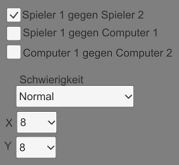
\includegraphics{img/Spieloptionen2}
	\caption{Spieloptionen}
	\label{fig:Spieloptionen}
\end{figure}
%% ==============================
\section{Verhalten in der Simulation ohne Analyse der Ausgangssituation}
%% ==============================
\label{ch:Evaluierung:sec:Simulation}
Zur Analyse des Simulationsverhalten wurden verschiedene Konfigurationen ausprobiert und beobachtet. Die erste Einstellung hat eine Suchtiefe von 3 und folgende Punkteverteilung: \\
\paragraph{Spieler 1 (Muscheln):}
\begin{itemize}
	\item Angriffspunkte: 80
	\item Verteidigungspunkte: 50
	\item Bedrohungspunkte: 20
	\item Hohe Bedrohungspunkte: 0
\end{itemize}

\paragraph{Spieler 2 (Steine):}
\begin{itemize}
	\item Angriffspunkte: 100
	\item Verteidigungspunkte: 20
	\item Bedrohungspunkte: 50
	\item Hohe Bedrohungspunkte: 80
\end{itemize}
Beide KIs wirken mit diesen Einstellungen sehr aggressiv. Der erste Zug eines Spiels, ist einer auf ein Feld ohne Feindkontakt. Anschließend bedroht der zweite Spieler die bewegte Figur, indem der Spielstein sich unmittelbar daneben platziert. Im nächsten Zug wird der zuletzt bewegte Stein erobert. Insgesamt wirkt die KI auf beiden Seiten als würde sie möglichst viele gegnerische Figuren bedrohen und angreifen wollen, auch wenn es eine eigene Bedrohung zur Folge hat. Außerdem fällt auf, dass die Muscheln mehr Eroberungen erreichen. Hier lässt sich festhalten, dass in 7 von 10 Spielrunden die Muscheln gewonnen haben. Allerdings wird erkennbar, dass die Steine durch das zusätzliche Flag Bedrohungen der Muscheln einleiten, die dadurch theoretisch im nächsten Zug erobert werden könnten.
\paragraph{Suchtiefe: 10}
Bei selber Konfiguration wie zuvor, aber erhöhter Suchtiefe, fällt auf, dass die Steine  auch versuchen Muscheln zu bedrohen, die nicht in einem Zug erreichbar sind. Dieses Verhalten führt allerdings auch dazu, dass die Muscheln diesen zusätzlichen Zug teilweise ausnutzen, um die bewegte Figur zu erobern. Die Gewinnchance bei 10 gespielten Runden ist gleich verteilt, sodass beide jeweils 5 gewonnen haben. Aufgefallen ist dabei, dass es gegen Ende des Spiels zu Situationen kommen kann, in denen beide Spieler ihre verbliebenen Steine (hier waren es jeweils zwei) immer wieder hin und her bewegen, ohne dabei zu einem Angriff zu kommen. Die KIs bewerten die Bedrohungen in so einer Situation so hoch, dass sie sich dadurch zuerst scheinbar ,,festfahren''.
\paragraph{Erhöhte Verteidigungspunkte und verminderte Angriffspunkte mit Suchtiefe 3}
\paragraph{Spieler 1 (Muscheln):}
\begin{itemize}
	\item Angriffspunkte: 80
	\item Verteidigungspunkte: 50
	\item Bedrohungspunkte: 20
	\item Hohe Bedrohungspunkte: 70
\end{itemize}
\paragraph{Spieler 2 (Steine):}
\begin{itemize}
	\item Angriffspunkte: 20
	\item Verteidigungspunkte: 100
	\item Bedrohungspunkte: 50
	\item Hohe Bedrohungspunkte: 80
\end{itemize}
Für die folgende Beobachtung wurden die Verteidigungspunkte der Steine mit den Angriffspunkten der ersten Konfiguration vertauscht und den Muscheln wurde ebenfalls das Flag der Hohen Bedrohung mitgegeben. Die beobachteten 10 Runden endeten jedes mal mit einem Sieg der Muscheln. Dabei ist aufgefallen, dass das Verteidigungs-Flag Wirkung zeigt und die Steine sich aus Bedrohungen zurückziehen. Allerdings führt das weniger aggressive Verhalten dazu, dass die Steine im Endeffekt die Runden verlieren. Außerdem gab es die Situation aus Abbildung \ref{fig:nicht erkannt}, in der die Muscheln nicht erkannt haben, dass die Steine eingekesselt werden können und somit das Spiel gewonnen wäre. Die Spieler haben ihre Spielsteine so lange bewegt, bis es für die Muscheln möglich war, einen zu erobern und dadurch das Spiel zu gewinnen.
\begin{figure}[h]
	\centering
	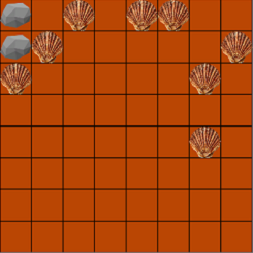
\includegraphics{img/einkesselnHidezuhoch2}
	\caption{Spielende wird nicht erkannt}
	\label{fig:nicht erkannt}
\end{figure}
\paragraph{Suchtiefe 10}
Bei erhöhter Suchtiefe haben die Steine 4 von 10 Runden gewonnen. Hier ist aufgefallen, dass mehr Angriffe über 2 Züge stattfinden. Dieses Verhalten kann auf die erhöhte Suchtiefe zurückgeführt werden. Dadurch können zukünftige Züge evaluiert werden und so Eroberungen die in späteren Zügen erst möglich sind durchgeführt werden. Insgesamt erweckt die KI allerdings den Eindruck, dass sie möglichst oft versucht gegnerische Spielsteine zu erobern. Aufgrund des zu aggressiven Verhaltens wurde die Analyse der Ausgangssituation implementiert, sowie weitere Flags für eine präzisere Bewertung.

%% ==============================
\section{Verhalten der KI ohne Analyse der Ausgangssituation gegen einen menschlichen Spieler}
%% ==============================
\label{ch:Evaluierung:sec:KIvsHuman}
\paragraph{Spieler 2 (Steine):}
\begin{itemize}
	\item Angriffspunkte: 100
	\item Verteidigungspunkte: 20
	\item Bedrohungspunkte: 50
	\item Hohe Bedrohungspunkte: 80
	\item Suchtiefe: 3
\end{itemize}
Die KI hat mit diesen Konfigurationen eine sehr aggressive Spielweise gezeigt. Dabei ist aufgefallen, dass vor allem die Bedrohung und Angriffe im Fokus stehen. Mit dieser Konfiguration war es möglich den Computer mit simplen Spielzügen aus der Verteidigung zu locken und die Steine zu erobern. Es wurden regelmäßig Steine neben Muscheln platziert, auch wenn es im nächsten Zug eine eigene Eroberung zur Folge hat. Der Verteidigungsmechanismus kommt in dieser Konfiguration nur selten zur Geltung. Einerseits sind dazu die defensiven Punkte zu gering angesetzt, sodass diese kaum Auswirkungen auf die Spielzüge haben, andererseits wurde hier auch eine geringe Suchtiefe gewählt, sodass die Verteidigung noch weniger ins Gewicht fällt und somit kaum Relevanz im Spiel zeigt. Um zu sehen, ob sich das Verhalten ändert, wurde die Suchtiefe auf 10 erhöht.

\paragraph{Spieler 2 (Steine):}
\begin{itemize}
	\item Angriffspunkte: 100
	\item Verteidigungspunkte: 20
	\item Bedrohungspunkte: 50
	\item Hohe Bedrohungspunkte: 80
	\item Suchtiefe: 10
\end{itemize}

Mit dieser Konfiguration wirkte die KI noch immer sehr aggressiv und hat kaum eine Möglichkeit ausgelassen, die Muscheln anzugreifen. Diese wurden in der Regel schnell wahrgenommen und umgesetzt, sodass allerdings im nächsten Zug wieder der angreifende Stein erobert werden konnte. Allerdings führten ein paar Bedrohungen dazu, dass die KI sich zurückgezogen und neben einem eigenen Stein eingereiht hat und nun nicht mehr so einfach einzunehmen war. Insgesamt wurde das Spielverhalten nach wenigen Runden vorhersehbar und konnte leicht überlistet werden.

\paragraph{Spieler 2 (Steine):}
\begin{itemize}
	\item Angriffspunkte: 80
	\item Verteidigungspunkte: 70
	\item Bedrohungspunkte: 50
	\item Hohe Bedrohungspunkte: 60
	\item Suchtiefe: 3
\end{itemize}
Für diese weiteren Tests wurden die Punktzahlen angepasst. Dabei wurden die Angriffs- und Bedrohungspunkte etwas reduziert und die Verteidigungspunkte erhöht, um dem defensiven Verhalten eine höhere Gewichtung zu geben. Diese Punkteverteilung machte sich auch im Verhalten bemerkbar. Die KI hat nicht mehr auf jede bewegte Muschel reagiert und sich so auch in der Verteidigung gehalten, allerdings wird schnell klar, dass dieses Verhalten zu passiv war und die Steine schnell eingekesselt werden konnten, sodass kein weiterer Zug mehr möglich war. Die KI hat eigene Bedrohungen noch immer nicht erkennen können, hat dafür aber nicht mehr auf jede Möglichkeit sich den Muscheln zu nähern reagiert. Anschließend wurde wieder die selbe Konfiguration mit der Suchtiefe 10 betrachtet.

\paragraph{Spieler 2 (Steine):}
\begin{itemize}
	\item Angriffspunkte: 80
	\item Verteidigungspunkte: 70
	\item Bedrohungspunkte: 50
	\item Hohe Bedrohungspunkte: 60
	\item Suchtiefe: 10
\end{itemize}
Mit dieser Veränderung hat die KI es geschafft, weniger durchdachte Züge zum eigenen Vorteil zu nutzen und Muscheln zu erobern. Allerdings passierte dies auf Kosten der eigenen Steine. Die KI wirkt insgesamt noch immer aggressiv und verliert in der Regel gegen geübte Spieler. Insgesamt hat sich gezeigt, dass die entwickelte KI noch zu primitiv ist und eigene Bedrohungen nicht zu erkennen scheint.\\
Daher wurden für weitere Analysen zusätzliche Kriterien implementiert, die unter anderem auch die aktuelle Spielsituation besser beschreiben und eigene Bedrohungen erkennen lassen. Das heißt, es wurde die Möglichkeit implementiert zu erkennen, dass ein Angriff zu eigenen Bedrohungen führen kann. Weiterhin wurden Situationen integriert, die dafür sorgen sollen, dass die Steine sich auch in Vierer-Formationen platzieren können. Diese zählen zu den stärksten Zügen in diesem Spiel, da es schlicht nicht möglich ist Spielsteine aus dieser Formation zu erobern. Weiterhin wurden Positionen am Rand des Spielbretts und vor allem die Ecken höher priorisiert. Um das ganze System von der Situation abhängig machen zu können, wurden Multiplikatoren als Gewichtung eingesetzt, die während der Evaluierung variieren können.
%% ==============================
\section{Verhalten in der Simulation mit Analyse der Ausgangssituation}
%% ==============================
\label{ch:Evaluierung:sec:SimulationWithAnalyse}
Für die folgenden Beobachtungen wurde die Simulation mit zusätzlichen gewichteten Analysekriterien betrachtet. Dabei gelten bei den ersten Tests die gleichen Punkteverteilungen für beide KIs und eine Suchtiefe von 10. Die Punkteverteilung entspricht der Abbildung~\ref{fig:punkteverteilung}.\\
Dies spiegelt sich stark in ihrem Verhalten wieder. Sowohl die Steine, als auch die Muscheln finden sehr schnell die wichtigen Positionen um nicht geschlagen zu werden. Haben beide Ihre unschlagbaren Positionen gefunden, dann bewegen sie sich nur noch zwischen den Verteidigungspositionen hin und her wie in Abbildung \ref{fig:hinundher} zu sehen ist. Dieses Verhalten hat sich endlos wiederholt.
\begin{figure}[h]
	\centering
	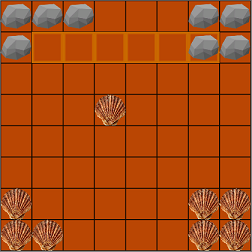
\includegraphics{img/mitAnalyse/hinundherCorner}
		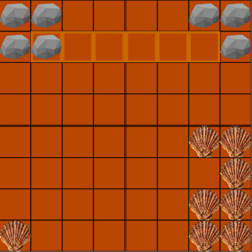
\includegraphics{img/mitAnalyse/hinundherCorner3}
	\caption{Steine und Muscheln mit der gleichen defensiven Konfiguration:\newline Links mit Suchtiefe 10 (Runde 7) und rechts mit Suchtiefe 3 (Runde 10)}
	\label{fig:hinundher}
\end{figure}

Zum Vergleich wurde diese Konfiguration mit angepasster Suchtiefe auf 3 übernommen und ebenfalls als Simulation getestet. Aufgefallen ist, dass beide KIs ein paar Züge mehr benötigen, um diese Eck-Positionen, wie in Abbildung \ref{fig:hinundher} zu sehen, zu finden und sich dort zu positionieren. Hier hat sich ebenfalls herausgestellt, dass diese Reduzierung nur dazu führt, die wichtigen Positionen später zu finden. Das Verhalten hat sich abgesehen von der längeren Suche nicht verändert.
Daran wird deutlich, dass es nicht sinnvoll ist die KIs mit gleicher defensiver Konfiguration als Simulation laufen zu lassen. Hier kann man sich zwar wichtige Positionen verdeutlichen, allerdings nichts darüber hinaus, da das Spiel so auch nicht enden wird. Für den folgenden Testlauf wurden die Punkte für die Angriffs-Flags erhöht und beobachtet.
\paragraph{Erhöhte Angriffs- und verminderte Verteidigungspunkte mit Suchtiefe 10}
Bei einer Suchtiefe von 10 und der selben Punkteverteilung für \textbf{beide} KIs  fällt auf, dass die Muscheln zu Beginn sich eher in die Mitte des Felds bewegen, die Steine sich aber recht zügig in die Eckpositionen begeben. Dabei bilden die Muscheln Reihenformationen, die eine wichtige strategische Formation im Spiel bilden, da die Steine nur noch von 2, statt von 4 Seiten angegriffen werden können. Die Simulation endet hier mit weniger aktiven Spielsteinen als im Test zuvor, allerdings fahren sich beide Spieler zum Ende hin wieder in den Eckpositionen fest.
\begin{figure}[h]
	\centering
	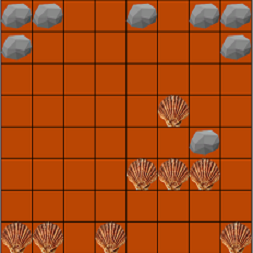
\includegraphics{img/reihe22}
	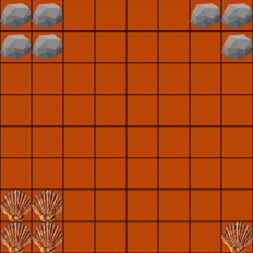
\includegraphics{img/Aggro/aggroEnde22}
	\caption{Steine und Muscheln mit der gleichen aggressiven Konfiguration und Suchtiefe 10: Links: Reihenformation \& rechts: Endsituation.}
	\label{fig:aggro}
\end{figure}
\paragraph{Erhöhte Angriffs- und verminderte Verteidigungspunkte mit Suchtiefe 3}
Bei diesen Einstellungen merkt man schnell, dass es länger dauert die Superpositionen zu finden. Die Spielsteine bewegen sich zuerst in die Mitte des Feldes, finden allerdings noch ihre verbündeten Steine, sodass sie sich nicht alleine offen ins Feld begeben. Allerdings tendieren sie nach wenigen Zügen dazu, sich wieder in die Ecken zu bewegen. Dabei stechen immer mal wieder Angriffe oder zumindest Angriffsversuche heraus. Zum Simulationsende hin fällt auf, dass immer wieder Versuche zur Bedrohung stattfinden, allerdings werden diese im darauffolgenden Zug wieder durch einen Rückzug hinfällig und die KIs befinden sich in einer Endlosschleife aus Bedrohung \& Rückzug, wie es in der Abbildung \ref{fig:aggro3} zu sehen ist.
\begin{figure}[h]
	\centering
	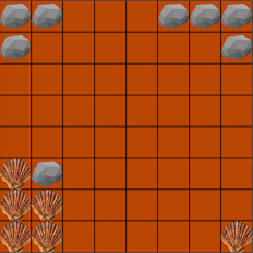
\includegraphics{img/Aggro/tiefe3Bedrohung2}
	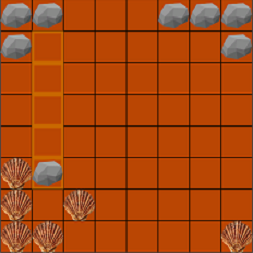
\includegraphics{img/Aggro/tiefe3rueckzug2}
	\caption{Steine und Muscheln mit der gleichen aggressiven Konfiguration und Suchtiefe 3: Endsituation.}
	\label{fig:aggro3}
\end{figure}

\paragraph{Flags mit ausgeglichener Punkteverteilung und Suchtiefe 10}
Bei diesem Versuch wurden die verschiedenen Flags mit der gleichen Punktzahl belegt. Dabei ist aufgefallen, dass das Spiel insgesamt weniger intelligent verläuft und die Spielsteine sich teilweise in bedrohliche Positionen begeben. Gute Positionen werden noch immer erkannt, allerdings scheinen die KIs direkte Bedrohungen immer identifizieren zu können. Vorteilhaft an dieser Konfiguration ist, dass es bei Vorführungszwecken unwahrscheinlicher wird, dass die Simulation sich in einer Situation festfährt und keiner der beiden gewinnt. Insgesamt erkennt man trotzdem noch, dass Positionen neben verbündeten Steinen eher aufgesucht werden als offene mitten im Spielfeld. Teilweise stellt die KI sich neben gegnerische Steine, wird aber im darauffolgenden Zug erobert. 

\paragraph{Flags mit ausgeglichener Punkteverteilung und Suchtiefe 3}
Mit verminderter Suchtiefe wirkt das Spielgeschehen noch zufälliger. Gute Positionen wie die Eckpunkte werden erkannt, genauso wie Positionen am Rand des Spielfelds und neben verbündeten Steinen. Allerdings fällt hier wieder auf, dass akute Bedrohungen nur noch teilweise erkannt werden. Wie zuvor mit der Suchtiefe 10 begeben sich die Steine in eine Bedrohungsposition, auch wenn im nächsten gegnerischen Zug die Steine erobert werden können. Stellenweise wirkt es, als würden Spielsteine des Gegners auf der eigenen Seite nicht erkannt werden. Hier bewegen sich die Steine ein paar Runden lang hin und her, wie in Abbildung \ref{fig:hinundherboth} bis die Muschel erobert wird.
\begin{figure}[h]
	\centering
	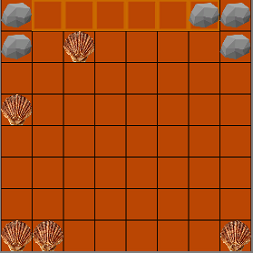
\includegraphics{img/both/muschelnichterkannt}

	\caption{Steine und Muscheln mit der gleichen Konfiguration und Suchtiefe erkennen mögliche Eroberung spät.}
	\label{fig:hinundherboth}
\end{figure}

\begin{figure}
	\begin{tabular}[h]{l|c|c|c}
		Flag & Ausgeglichene Punkte & Erhöhter Angriff & Erhöhte Verteidigung \\
		\hline
		Attack & 50 & 100 & 100\\
		Hide & 50 & 10 & 20\\
		Threat & 50 & 70 & 10\\
		HighThreat & 50 & 80 & 60\\
		Squad & 40 & 20 & 40\\
		prepSquad & 50 & 10 & 20 \\
		corner & 50 & 10 & 100\\
		FriendlyCorner & 20 & 20 & 20\\
		HighAlert & -50 & -100 & -100\\
	\end{tabular}
	\caption{Punkteverteilung im Spiel gegen die KI}
	\label{fig:punkteverteilung}
\end{figure}

\paragraph{Aggressive gegen Defensive KI}
Lässt man die aggressive gegen die defensive Konfiguration spielen, werden die Spielmechaniken deutlicher. Die defensive KI wirkt insgesamt stärker und sucht sich schnell gute Spielpositionen in den eigenen Ecken. Die Aggressive versucht vor allem zu Beginn noch oft Steine zu erobern, verliert bei dem Versuch aber oft eigene. Allerdings orientiert sich diese auch mit steigender Rundenzahl in die Ecken und an den eigenen Steinen. In diesem Versuch gewinnt die Defensive KI, da sie sich seltener in Positionen begibt, in denen eigene Steine erobert werden können. Zur Vorführung scheint diese Einstellung am sinnvollsten, da Spielmechaniken wie Eroberungen und Verteidigungen klar werden. 
%% ==============================
\section{Verhalten der KI mit Analyse der Ausgangssituation gegen einen menschlichen Spieler}
%% ==============================
\label{ch:Evaluierung:sec:KIvsHumanWithAnalyse}
Die nachfolgenden Beobachtungen wurden bei einer Suchtiefe von 10 und mit den Konfigurationen aus der Abbildung~\ref{fig:punkteverteilung} gemacht. Bei erhöhten Verteidigungspunkten und der Analyse des aktuellen Spielzustands hat das Spiel im Vergleich zu den Tests ohne Betrachtung der gegenwärtigen Situation bereits an Schwierigkeit gewonnen. Die Rolle der Steine wurde von der KI übernommen, wohingegen die Muscheln von mir gesteuert wurden. Die KI macht einen intelligenteren Eindruck und lässt sich nicht mehr bei jeder Gelegenheit erobern. Weiterhin fällt hier auf, dass der Computer sich nach Angriffen auch wieder in eine sichere Position zurückzieht. Außerdem lassen die Steine sich auch nicht mehr aus ihrer Deckung locken, indem man die Muscheln einfach auf den mittleren horizontalen Reihen des Spielfelds zieht.\\
Betrachtet man die Konfiguration mit verminderter Verteidigungs- und erhöhter Angriffsgewichtung, scheint das Spielen gegen die KI schwerer zu werden. Die Steine ziehen sich immer wieder in die Eckpositionen zurück und versuchen in den meisten Fällen nur anzugreifen, wenn der Angriff nach Berechnung auch sicher ist. Diese Konfiguration wirkt sinnvoller als in der Simulation mit gleicher Punkteverteilung für beide KIs aus dem Kapitel~\ref{ch:Evaluierung:sec:SimulationWithAnalyse}. Das Verhalten lässt sich so erklären, dass bei gleicher Punkteverteilung beide KIs versuchen ihre Spielsteine zu schützen und es nur selten zu Bedrohungen oder Angriffen kommt. Die KIs ziehen sich zurück, sobald erkannt wird, dass ein Angriff auf den Stein möglich ist. Da menschliche Spieler dazu tendieren können, die gegnerischen Spielsteine zu erobern, kommt der Verteidigungsmechanismus des Computers mehr zur Geltung.


\paragraph{Erhöhte Angriffs- und verminderte Verteidigungspunkte mit Suchtiefe 10}
Die KI hat sich mit diesen Einstellungen einmauern lassen und so das Spiel schnell verloren. Insgesamt fällt auf, dass weniger defensiv gespielt wird als zuvor. Sie bewegt sich die meiste Zeit auf der eigenen Startseite, nutzt aber die Position clever aus, wenn sich ein Stein auf die gegnerische Spielseite bewegt hat. Die erhöhte Gewichtung der Angriffspunkte führt stellenweise zu Zügen in denen bis zu 3 Steine von mir erobert wurden.
\paragraph{Erhöhte Angriffs- und verminderte Verteidigungspunkte mit Suchtiefe 3}
Bei geringerer Suchtiefe hat sich die KI durch ein aggressives Verhalten von mir schnell besiegen lassen. Bedrohungen wurden zwar erkannt, allerdings hat der Computer vor allem mit vielen Spielsteinen auf dem Feld sich seltener dafür entschieden, eine Bedrohung nicht einzugehen, wenn im nachfolgenden Zug der bewegte Stein erobert werden kann. Dieses Verhalten lässt sich auf die geringe Suchtiefe zurückführen. Gegen Ende des Spiels ist die Situation aus der Abbildung \ref{fig:nichtschlagbar} aufgefallen. Die KI hat sich nur noch in den Eckpositionen bewegt und hat sich nicht mehr in eine Situation bringen lassen, in der ich einen Stein erobern konnte.
\begin{figure}[h]
	\centering
	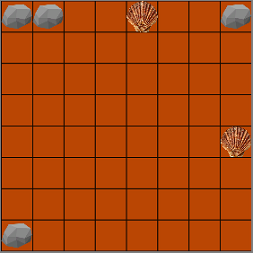
\includegraphics{img/Aggro/humannichtzuschlagen2}	
	\caption{Hohe Angriffspunkte bei Suchtiefe 3. KI weicht in die Ecken aus.}
	\label{fig:nichtschlagbar}
\end{figure}
\paragraph{Ausgeglichene Punkteverteilung}
Diese Einstellungen werden hauptsächlich durch die Gewichtung via Multiplikatoren beeinflusst. Das fällt auch im Spiel auf. Die Züge wirken teilweise nicht zielführend, wie zum Beispiel, wenn man sich neben einen computer-gesteuerten Stein platziert, entscheidet sich die KI stellenweise dafür diesen Stein durch eine Eroberung zu verlieren und bringt ihn nicht in Sicherheit. In der Abbildung \ref{fig:humaneingekesselt} erkennt man ein großes Problem bei diesen Einstellungen. Die KI hat sich zu Beginn des Spiels auf der eigenen Spielseite einkesseln lassen, sodass es nach nur einer Eroberung beendet war. Diese Situation entsteht dadurch, dass die KI sich mit ihrem ersten bewegten Stein nur eine Position nach vorne bewegt. Anschließend wird der Stein nur noch horizontal von einer Ecke zur nächsten geschoben. Diese Konfiguration ist bis hierhin die am wenigsten zielführende. Mit geringerer Suchtiefe lässt die KI sich ebenfalls wie in der Abbildung \ref{fig:humaneingekesselt} einkesseln und verliert dadurch das Spiel. Insgesamt wirkt diese Konfiguration sehr zurückhaltend, da die KI kaum versucht gegnerische Steine zu erobern.
\begin{figure}[h]
	\centering
	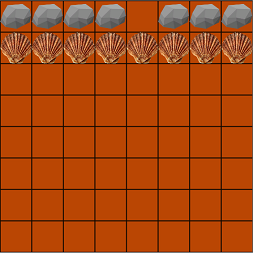
\includegraphics{img/both/humaneingekesselt}	
	\caption{KI lässt sich einfach einmauern.}
	\label{fig:humaneingekesselt}
\end{figure}

\par Zusammenfassend kann man festhalten, dass die KI sich gegen menschliche Spieler mit der defensiven Konfiguration aus der Abbildung~\ref{fig:punkteverteilung} am besten geschlagen hat. Die KI begibt sich meistens nur aus sicheren Positionen heraus, wenn eine Eroberung möglich ist ohne dadurch die eigenen Steine zu verlieren. Daher wurde diese Einstellung als schwer eingestuft. Die aggressiv eingestellte KI hat sich leicht einmauern lassen und begibt sich öfter in Situationen, die zu einer leichten Eroberung der eigenen Steine führt. Da eine ausgeglichene Punkteverteilung zu einem wenig zielführenden Verhalten geführt hat, wurde diese als leicht klassifiziert und die aggressive als mittlerer Schwierigkeitsgrad.
%\paragraph{Flags mit gleicher Punkteverteilung und Suchtiefe 3}


%Bei erhöhter Suchtiefe 
%% ==============================
%\section{Zusammenfassung}
%% ==============================
%\label{ch:Evaluierung:sec:zusammenfassung}

%Am Ende sollten ggf. die wichtigsten Ergebnisse nochmal in \emph{einem} kurzen Absatz zusammengefasst werden.

%%% Local Variables: 
%%% mode: latex
%%% TeX-master: "thesis"
%%% End: 
